%   % !TEX root = ../../VIII,3_Rahmen-TeX_9-0.tex
%  
%   Band VIII, 3 N.~?? 	[STO??.?]			(Unter)rubrik			??
%   Signatur/Tex-Datei:	LH_37_05_148-149
%   RK-Nr. 	57276
%   Überschrift: 	(keine)
%   Titel: 			??			(unser Titel)					??
%   Datierung:		???? bis ????								??
%   Textfolge: 			149r+v, 148r+v
%   WZ: 	im Falz, Nr. 803017 	(Fragment)				
%   edlabels: 			11 (+ 1 für PR zw. Querverweis)
%   Diagramme: 		6 (eigtl. 5)
%   Dateien (PDF):
%   		LH_37_05_148-149_d1_149r.pdf;		gehört eigtl zu 37 5 140-141; dorthin verlegt
%   		LH_37_05_148-149_d2_149r.pdf;						
%   		LH_37_05_148-149_d3_149v.pdf;						
%   		LH_37_05_148-149_d4_149v.pdf;						
%   		LH_37_05_148-149_d5_148r.pdf;						
%   		LH_37_05_148-149_d6_148v.pdf.
%
%   Erstaufnahme:			Bayuk 2014
%   Bearbeitung MS ab: 		Juli 2019
%
%   NB: 	Bl. 148 beschnitten (halbiert); Figur 149 gehört vllt zu 140?  USF.	??
%
%
%
\selectlanguage{ngerman}
\frenchspacing
%
\begin{ledgroupsized}[r]{120mm}
\footnotesize
\pstart
\noindent\textbf{Überlieferung:}
\pend
\end{ledgroupsized}
%
\begin{ledgroupsized}[r]{114mm}
\footnotesize
\pstart \parindent -6mm 
\makebox[6mm][l]{\textit{L}}% %%
Konzept: 
LH~XXXVII~5 Bl.~148\textendash149. 
Ein Bogen 4\textsuperscript{o};
Bl.~148 ist halbiert;
Wasserzeichenfragment im Falz;
Ränder ausgefranst; Papiererhaltungsmaßnahmen.
Vier Seiten;
Textfolge: Bl.~149, dann Bl.~148;
der obere Bereich von Bl.~149~r\textsuperscript{o} überliefert die \lbrack\textit{Fig.~1}\rbrack\ von N.~\ref{RK57275}.
\pend
\end{ledgroupsized}
%
\begin{ledgroupsized}[r]{114mm}
\footnotesize
\pstart
\parindent -6mm 
\makebox[6mm][l]{\textit{E}}% %%
(tlw.) \cite{01056}\textsc{Fichant} 1994, S.~397f.
\pend
\end{ledgroupsized}
%
%
\vspace{5mm}
\begin{ledgroup}
\footnotesize
\pstart
\noindent
\textbf{Datierungsgründe:} %
Im vorliegenden Konzept behandelt Leibniz die Bewegung des gemeinsamen Schwerpunkts der Körper beim Stoß
%
anhand der Schiffsanalogie, die erst in N.~\ref{RK57269} vom 10.\ (20.) Juni 1677 
%
behandelt wurde. Damit ist ein erster Grund zur Annahme der Entstehung von N.~\ref{RK57276} nach N.~\ref{RK57269} gegeben.
%
Ein wesentlicher Unterschied zu N.~\ref{RK57269} besteht darin,  
%
dass Leibniz dort diese Analogie zunächst als anschauliches Beispiel der Gefahren dieser Vorgehensweise angeführt hatte, 
um anschließend ihre Bedeutung für die Stoßanalyse zu erörtern.
%
In N.~\ref{RK57276} jedoch weicht sein Misstrauen gegen die auf dem Relativitätsprinzip beruhende Methode 
einer gegensätzlichen Haltung:
%
Leibniz nennt die Methode \glqq compositionem motuum meam\grqq\ (S.~\refpassage{37_05_148-149_9a}{37_05_148-149_9b}) 
und \glqq regula nostra per compositiones\grqq\ (S.~\refpassage{37_05_148-149_10a}{37_05_148-149_10b})
%
und verwendet sie als Maßstab zur Beurteilung der \protect\index{Namensregister}{\textso{Huygens} (Hugenius, Ugenius, Hugens, Huguens), Christiaan 1629\textendash1695}Huygens'schen Stoßregeln.
%
Dies deutet auf eine Entwicklung von Leibnizens Position nach der Abfassung von N.~\ref{RK57269} und spricht für
%
die Enstehung von N.~\ref{RK57276} ab Ende Juni 1677.
%
Leibnizens Bedenken über die unerwünschten Folgen der Schiffsmethode hinsichtlich der Erhaltung der \textit{potentia} bleiben allerdings bestehen (S.~\refpassage{37_05_148-149_11a}{37_05_148-149_11b}) und sind Gegenstand weiterer Untersuchungen
%
(N.~\ref{RK57275} und N.~\ref{RK57272}).
\pend
%
\pstart
Als Terminus ante quem darf  \textit{De corporum concursu}, \textit{Scheda octava}  von Januar 1678 (N.~\ref{dcc_08}) gelten.
%
Denn Leibniz sieht in N.~\ref{RK57276}, wie auch in N.~\ref{RK57275}, das Hauptproblem seiner 
%
(aus heutiger Sicht grundsätzlich richtigen) Stoßregel \glqq per compositiones\grqq\ darin, dass 
%
sie die Erhaltung der gesamten \textit{potentia} der Körper wider Erwarten nicht gewährleistet
(S.~\refpassage{37_05_148-149_11a}{37_05_148-149_11b}).
%
Der Grund dafür ist, dass er unter \textit{potentia} die skalare Größe $mv$ versteht, die im Gegensatz zum (vektoriellen) Impuls beim Stoß nicht erhalten wird.
%
In der \textit{Scheda octava} wird Leibniz eine \glqq reformatio\grqq\  der Stoßlehre vollziehen,
%
die Erhaltungssätze für den Impuls und für die dort erstmals als $mv^2$ gemessene \textit{vis} umfasst,
%
wodurch die hier geäußerten Bedenken über die Nichterhaltung der Bewegungsgröße sich als gegenstandslos erweisen.
%
%
\pend
%
\pstart
Die thematischen und inhaltlichen Übereinstimmungen zwischen N.~\ref{RK57276} und N.~\ref{RK57275} 
legen die Annahme einer etwa gleichzeitigen Entstehung beider Stücke nahe,
%
welche durch folgenden Umstand bestätigt und präzisiert wird.
%
Der obere Bereich von Bl.~149~r\textsuperscript{o} überliefert eine Zeichnung, die nicht zu N.~\ref{RK57276} gehört, sondern
%
die Grundlage für die Fallanalyse dreier Stoßfälle in N.~\ref{RK57275} bildet
%
(und dementsprechend dort als \lbrack\textit{Fig.~1}\rbrack\ wiedergegeben wird).
%
Die Lage der Figur lässt den Schluss zu, dass Leibniz nach Anfertigung von N.~\ref{RK57276} 
%
sie am frei gebliebenen Rand von Bl.~149~r\textsuperscript{o} zeichnete und anschließend
%
zur Abfassung von N.~\ref{RK57275} ansetzte.
\pend
\end{ledgroup}
%
\newpage
%
\selectlanguage{latin}
\frenchspacing
\vspace{8mm}
\pstart%
\normalsize%
\noindent%
\lbrack149~r\textsuperscript{o}\rbrack\ \pend
\vspace{1.0em} 
  \centerline{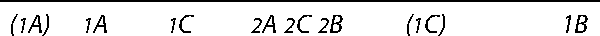
\includegraphics[width=0.66\textwidth]{gesamttex/edit_VIII,3/images/LH_37_05_148-149_d1_149r.pdf}} 
    \vspace{0.5em}
\centerline{\lbrack\textit{Fig.~1}\rbrack}
% \newpage%
  \vspace{1.5em}
\pstart \noindent
%
Videndum an centrum gravitatis\protect\index{Sachverzeichnis}{centrum gravitatis} semper in eam partem tendat \edtext{ante concursum\protect\index{Sachverzeichnis}{concursus}}{\lemma{}\Bfootnote{ante concursum \textit{erg.}~\textit{L}}} in quam tendit corpus 
%
fortius\protect\index{Sachverzeichnis}{corpus fortius}. Fortius
%
% = 
voco non majus\protect\index{Sachverzeichnis}{corpus majus}, sed cujus potentia\protect\index{Sachverzeichnis}{potentia} major. Nempe sit  
%
\edtext{celeritas \textit{B} seu ${\scriptstyle \textit{1}}B{\scriptstyle \textit{2}}B \sqcap f$. $bf\, \groesser\, ae$. Et}{\lemma{celeritas \textit{B}}\Bfootnote{\textit{(1)}~$\sqcap\ f$. Distantia ejus a \textit{{\scriptsize 2}B} \textit{{\scriptsize 1}B{\scriptsize 2}B} sit \textit{(a)}~; \textit{a} erit \textit{e} \textit{(b)}~et alterius distantia \textit{\scriptsize 1} \textit{(2)}~seu ${\scriptstyle \textit{1}}B{\scriptstyle \textit{2}}B \sqcap f$. \textit{(a)}~$fb\ \groesser$ \textit{(b)}~$bf\ \groesser\ ae$. \textit{(aa)}~Ergo \textit{e} \textit{(bb)}~Et~\textit{L}}}
%
\protect\rule[0cm]{0mm}{12pt}\edtext{$e+f\, \sqcap\, la+lb$. Est autem $f\, \sqcap\, la+lb-e$. Ergo $bf\, \sqcap\, bla+lb^2-be$. Quem valorem \textit{bf} in determinatione $bf\ \groesser\ ae$ substituendo erit $bla + lb^2 - be\ \groesser\ ae$, seu $bla + lb^2\ \groesser\ ae+be$, seu $bl\ \groesser\ e$. Ergo semper erit $bl\ \groesser\ e$. Et eodem modo quia}%
{\lemma{$e+f \sqcap la+lb$.}%
\Bfootnote{\textbar\ (\phantom)\hspace*{-1.2mm}Quaeritur an $f\,\groesser\,bl$ \textit{erg. u. gestr.}~\textbar\ Est \lbrack...\rbrack\ $bf \sqcap bla+lb^2-be$. \textit{(1)}~$bf\ \groesser$ \textit{(2)}~\textbar\ Ergo \textit{streicht Hrsg.}~\textbar\ substituendo in determinatione $bf\ \groesser\ a$ \textit{erg.}~\textbar\ \textit{(3)}~\textbar~Quem \lbrack...\rbrack\ erit \textit{erg.}~\textbar\ $bla + lb^2 - be\ \groesser\ ae$, \lbrack...\rbrack\ Ergo \textit{(a)}~si $f\ \groesser\ bl$ \textit{(b)}~semper erit $bl\ \groesser\ e$. \textit{(aa)}~Ergo \textit{(bb)}~Sed quaestio non erat an $f\ \groesser\ bl$, \textit{(aaa)}~seu \textit{(bbb)}~sed an $f\ \groesser\ al$\phantom(\hspace*{-1.2mm}). Quaeritur an $f\ \groesser\ al$. \textit{(cc)}~Et eodem modo \textbar\ et \textit{streicht Hrsg.}~\textbar\ quia~\textit{L}}}
%
$e\, \sqcap\, la+lb-f$ seu
% =
$ae\, \sqcap\, la^2+alb-af$, fiet $bf\ \groesser\ la^2+alb-af$. Seu $af+bf\ \groesser\ la^2+alb$
% =
seu dividendo utrobique per $a+b$, fiet: \edlabel{37_05_148-149_1a}$f\ \groesser\ \edtext{\lbrack la\rbrack}{\lemma{\textit{lb}}\Bfootnote{\textit{L ändert Hrsg.}}}$.\edlabel{37_05_148-149_1b} Seu 
%
semper ${\scriptstyle \textit{1}}B{\scriptstyle \textit{2}}B\ \groesser\ {\scriptstyle \textit{1}}B{\scriptstyle \textit{1}}C$, posito corpus \textit{B} esse potentius\protect\index{Sachverzeichnis}{corpus potentius}.
% =
\pend \pstart
Ergo centrum gravitatis\protect\index{Sachverzeichnis}{centrum gravitatis} 
%
\edtext{semper in eam}{\lemma{semper in}\Bfootnote{\textit{(1)}~eandem \textit{(2)}~eam~\textit{L}}}
%
tendit partem, in quam tendit corpus
%
\edlabel{37_05_148-149_2a}\edtext{}{% potentius: Varianten und Ergänzung!
{\xxref{37_05_148-149_2a}{37_05_148-149_2b}}%
\lemma{potentius.}\Bfootnote{\textbar~\textit{(1)}~Ut alia ejusmodi theoremata investigemus in determinatione $lfb\ \groesser\ lae$
%
tollamus \textit{lb}. Quaerendo valorem ipsius \textit{lb} per aequationem fiet $lb \sqcap e+f-la$,
%
et $lbf \sqcap ef+f^2-laf$ ergo $ef+f^2-laf\ \groesser\ ael$, seu $ef+f^2\ \groesser\ ael+laf$. Ergo $f\ \groesser\ al$. Nihil ergo hinc novi. \textit{(2)}~Via centri \lbrack...\rbrack\ in qua $a+b$ %
\textit{(a)}~(\phantom)\hspace*{-1.2mm}fingendo \textit{(b)}~ponendo haec esse distantias a centro gravitatis, \textit{(aa)}~minu \textit{(bb)}~seu corporum distantiam \textbar\ minuitur \textit{ändert Hrsg.}~\textbar\ \phantom(\hspace*{-1.2mm}), cum \lbrack...\rbrack\ 
manebit calculus \textit{(aaa)}~fitque \textit{(bbb)}~quia sublatis \lbrack...\rbrack\ est notabile. \textit{erg.}~\textbar\ \textit{(1)}~Si \textit{(2)}~Hinc si~\textit{L}}}% 
potentius.
\pend \pstart
\hspace{1mm}\hspace{-1mm}% Trick, weil \edlabel nicht zu \par-Beginn sein darf
\edlabel{LH_37_05_149r_pnctmtrl-1}%
Via centri gravitatis\protect\index{Sachverzeichnis}{via centri gravitatis} \textit{{\scriptsize 1}C{\scriptsize 2}C} sic investigabitur: nil refert etsi ponas corpora non in punctis esse, sed in momento concursus\protect\index{Sachverzeichnis}{momentum concursus} valde
% =
distare, quia ponendo \textit{l} esse rationem in qua $a+b$ \lbrack(\phantom)\hspace*{-1.2mm}\rbrack ponendo
%
haec esse distantias a centro gravitatis\protect\index{Sachverzeichnis}{distantia a centro gravitatis}, seu
%
corporum distantiam\protect\index{Sachverzeichnis}{distantia corporum} \lbrack minui\rbrack\phantom(\hspace*{-1.2mm}), cum $e+f$ (\phantom)\hspace*{-1.2mm}quae non est 
%
corporum distantia\protect\index{Sachverzeichnis}{distantia corporum} sed distantia illa, addita
%
distantia novissima\phantom(\hspace*{-1.2mm}) aequari debet, idem
%
manebit calculus\lbrack,\rbrack\ quia sublatis aliis in
% =
conclusione fit
%
\edtext{$f\ \groesser\ lb$,}{\lemma{$f\ \groesser\ lb$}%	%FN zur Ungleichung
\Cfootnote{Aus den Prämissen lässt sich nur die Ungleichung $f\ \groesser\ la$ folgern, nicht aber $f\ \groesser\ lb$. Es handelt sich wohl um eine Auswirkung des Fehlers auf S.~\refpassage{37_05_148-149_1a}{37_05_148-149_1b}.}} 
%
idque adhuc multo % =
%
magis, quia \textit{l} ponitur minuere. Elegans in hoc usus signorum\protect\index{Sachverzeichnis}{usus elegans signorum}, cum enim aliud nobis
% =
significet \textit{l}, hic ejus significationem mutando
% =
retento calculo intentum concludimus\lbrack,\rbrack\ quod est notabile.%
\edlabel{LH_37_05_149r_pnctmtrl-2}
\pend \pstart
Hinc si \edlabel{37_05_148-149_2b} %Ende EDLABEL
%
verum est centrum \edtext{gravitatis in easdem semper partes}{\lemma{gravitatis}\Bfootnote{\textit{(1)}~eadem semper \textbar\ recta \textit{streicht Hrsg.}~\textbar\ unifor \textit{(2)}~in easdem semper partes~\textit{L}}}
%
tendere\protect\index{Sachverzeichnis}{centrum gravitatis in easdem semper partes iens}, necesse est 
% =
per concursum\protect\index{Sachverzeichnis}{concursus} alternari fortitudines\protect\index{Sachverzeichnis}{fortitudo}, id est corpus quod erat
% =
fortius\protect\index{Sachverzeichnis}{corpus fortius} fieri debilius\protect\index{Sachverzeichnis}{corpus debilius} et  
%
\edtext{contra, id est fortioris\protect\index{Sachverzeichnis}{corpus fortius}}{\lemma{contra, id est}\Bfootnote{\textit{(1)}~mi \textit{(2)}~celerioris certitudinem \textit{(3)}~minui fortioris augeri \textit{(4)}~fortioris~\textit{L}}}
%
celeritatem minui (nam moles\protect\index{Sachverzeichnis}{moles} minui
% =
non potest), debilioris\protect\index{Sachverzeichnis}{corpus debilius} \edlabel{37_05_148-149_3a}\edtext{}{% NEUER ABSATZ UND VARIANTEN – "augeri. Calculavimus"
{\xxref{37_05_148-149_3a}{37_05_148-149_3b}}%
\lemma{augeri.}%
\Bfootnote{\textit{(1)}~Si ambo \textit{(2)}~Calculavimus~\textit{L}}}% 
augeri.
\pend \pstart
%
Calculavimus\edlabel{37_05_148-149_3b} ante
% =
tantum in eo casu, quo corpora sibi occurrant, quod si in easdem
% =
tendant partes, utique manifestissimum est, centrum
% 
\edtext{gravitatis\protect\index{Sachverzeichnis}{centrum gravitatis} ire}{\lemma{gravitatis}\Bfootnote{\textit{(1)}~tendere \textit{(2)}~ire~\textit{L}}}
%
cum utroque ergo et cum fortiore\protect\index{Sachverzeichnis}{corpus fortius}. Concursu\protect\index{Sachverzeichnis}{concursus} autem facto si adhuc in easdem
%
partes tendant utique tendit adhuc cum fortiore\protect\index{Sachverzeichnis}{corpus fortius}, si vero post concursum\protect\index{Sachverzeichnis}{concursus}
% =
in diversas tendant  
%
\edtext{partes, tunc}{\lemma{partes,}\Bfootnote{\textit{(1)}~quoniam \textit{(2)}~tunc si id quod \textit{(a)}~incurrit \textit{(b)}~ictum excepit \textbar\ est \textit{streicht Hrsg.}~\textbar\ fortius, utique patet \textit{(3)}~tunc~\textit{L}}}
%
nihilominus semper tendet in partem illam
% =
in quam tendit corpus excipiens\protect\index{Sachverzeichnis}{corpus excipiens}, quia corpus excipiens\protect\index{Sachverzeichnis}{corpus excipiens} semper tendit in
% =
easdem partes (nihil enim repellit) et centrum gravitatis\protect\index{Sachverzeichnis}{centrum gravitatis} etiam. Ergo
% =
post concursum\protect\index{Sachverzeichnis}{concursus} si corpora in diversas eant partes 
%
\edtext{erit corpus}{\lemma{erit}\Bfootnote{\textit{(1)}~centrum gravi \textit{(2)}~corpus~\textit{L}}}
% =
excipiens\protect\index{Sachverzeichnis}{corpus excipiens} fortius, positis quae dixi de gravitatis
% =
centro in easdem semper partes eunte\protect\index{Sachverzeichnis}{centrum gravitatis in easdem semper partes iens}.
\pend \pstart
\protect\rule[0cm]{0mm}{16pt}Hoc sine calculo patet, quia
\edtext{$bf\ \groesser\ ae$ seu $\displaystyle\frac{b}{a}\ \groesser\ \displaystyle\frac{e}{f}$}{\lemma{$bf\ \groesser\ ae$}\Bfootnote{\textit{(1)}~. Ergo  $\displaystyle\frac{b}{a}\ \groesser\ \displaystyle\frac{e}{f}$ \textit{(2)}~seu $\displaystyle\frac{b}{a}\ \groesser\ \displaystyle\frac{e}{f}$~\textit{L}}}  seu $\displaystyle\frac{a}{b}\ \kleiner\ \displaystyle\frac{f}{e}$ seu $ \displaystyle\frac{{\scriptstyle \textit{1}}B{\scriptstyle \textit{1}}C}{{\scriptstyle \textit{1}}A{\scriptstyle \textit{1}}C}\, $
%
\edlabel{37_05_148-149_4a}\edtext{}{% NEUER ABSATZ UND VARIANTEN – "$1b2b. +e+f"
{\xxref{37_05_148-149_4a}{37_05_148-149_4b}}%
\lemma{$\displaystyle\frac{{\scriptstyle \textit{1}}B{\scriptstyle \textit{2}}B}{{\scriptstyle \textit{1}}A{\scriptstyle \textit{2}}A}$.}%
\Bfootnote{\textit{(1)}~Hinc duobus corporibus \textit{(a)}~corpo \textit{(b)}~concurrentibus semper centrum gravitatis sequitur alteru \textit{(2)}~\lbrack149~v\textsuperscript{o}\rbrack\ $+e+f \sqcap i+m$.~\textit{L}}}% 
$\kleiner\ \displaystyle\frac{{\scriptstyle \textit{1}}B{\scriptstyle \textit{2}}B}{{\scriptstyle \textit{1}}A{\scriptstyle \textit{2}}A}$. \lbrack149~v\textsuperscript{o}\rbrack\
\pend
%%%%%%%%%%%%%%%%%%%%%%%%%%%%%%%%%%%%%%%%%%%%%%%%%%%%%%%%%%%
%%%%%%%%%%%%%%%%%%%%%%%%%%%%%%% FIG. 3 %%%%%%%%%%%%%%%%%%%%%%%%%%%%
\vspace{0.5em}
  \centerline{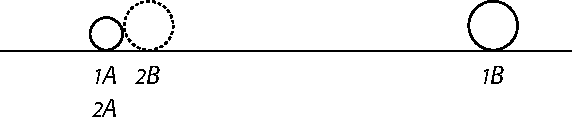
\includegraphics[width=0.66\textwidth]{gesamttex/edit_VIII,3/images/LH_37_05_148-149_d2_149v.pdf}} 
    \vspace{0.0em}
\centerline{\lbrack\textit{Fig.~2}\rbrack}
% \newpage%									
  \vspace{1em}
\pstart
$+e+f\, \sqcap\, i+m$.\edlabel{37_05_148-149_4b} $e-i\, \sqcap\, m-f$
et
$\displaystyle\frac{a}{b} \sqcap \displaystyle\frac{m-f}{e-i}$.
Ergo $ai\, \sqcap\, ae + af - am$ et rursus $ae+bf\, \sqcap\, ai+bm$ 
seu
$ai \sqcap ae+bf-bm$.
Ergo 
$\ovalbox{$ae$}+af-am \sqcap \ovalbox{$ae$}+bf-bm$.
%
Ergo $\overline{a-b}\,f \sqcap \overline{a-b}\,m$. Ergo $m\; \sqcap$
%
\edtext{$\displaystyle\frac{a-b}{a-b}\,f$. Ergo fiet}{\lemma{$\displaystyle\frac{a+b}{a-b}\,f$}\Bfootnote{\textit{(1)}~seu \textit{m} ad \textit{f} ut $a+b$ ut $a-b$. Ergo \textbar\ \textit{i} \textit{streicht Hrsg.}~\textbar\ \textit{(2)}~. Rursus $bm \sqcap be\;\protect\ovalbox{$+bf$}-bi \sqcap ae\;\protect\ovalbox{$+bf$}-ai$ \textit{(3)}~rursus \textit{(4)}~. Ergo \textit{(a)}~fieret \textit{(b)}~fiet~\textit{L}}}
%
vel 
$f \sqcap m$, 
quod excepto
% =
\protect\rule[0cm]{0mm}{16pt}uno casu absurdum, cum scilicet vires\protect\index{Sachverzeichnis}{vis} reciprocae,
% =
\protect\rule[0cm]{0mm}{10pt}vel fiet $a \sqcap b$. Aliis casibus semper necesse est
% =
ut si
%
\edtext{corpora occurrunt,}{\lemma{corpora}\Bfootnote{\textit{(1)}~concurrunt \textit{(2)}~occurrunt,~\textit{L}}}
%
unum sequatur 
\protect\rule[0cm]{0mm}{12pt}alterum. Faciamus ergo $e+f\; \sqcap$
% =
\edlabel{37_05_148-149_5a}\edtext{}{% A-Footnote und B-Footnote
{\xxref{37_05_148-149_5a}{37_05_148-149_5b}}%
\lemma{$\pleibdashv\; i\; \pleibvdash\; m$.}%
\Bfootnote{\textit{(1)}~Ergo \textit{(2)}~Ponamus~\textit{L}}}% 
\edtext{$\pleibdashv\; i\; \pleibvdash\; m$.}{\lemma{}\Afootnote{\textit{Neben} $e+f \sqcap\; \pleibdashv\; i\; \pleibvdash\; m$, \textit{in tlw.\ Überschneidung mit \lbrack Fig.~3\rbrack}:\enskip \textit{i}\textsuperscript{\lbrack a\rbrack} et \textit{m} non sunt aequales%
\newline\newline%Marginalienapparat
{\footnotesize \textsuperscript{\lbrack a\rbrack} \textit{i} \textit{(1)}~$+\,m$ \textit{(2)}~et \textit{m} non~\textit{L}}}}
%
Ponamus \edlabel{37_05_148-149_5b}
%
primum $e+f \sqcap i-m$.
Fiet
$m+f\, \sqcap\, i-e$.
%
Ergo
%
$e-i\, \sqcap\, -f-m$.
Ergo
$\displaystyle\frac{a}{b} \sqcap \displaystyle\frac{f-m}{f+m}$.
%
Ergo 
$af+am \sqcap bf-bm$.
Ergo
$\displaystyle\frac{bf-af}{a+b} \sqcap m$.
seu
$m \sqcap \displaystyle\frac{b-a}{a+b}\;f$.
% =
Ergo
%
\edtext{in casu occursus}{\lemma{}\Bfootnote{in casu occursus \textit{erg.}~\textit{L}}}
%
si \textit{i} sit major \textit{m} debet esse \textit{b} major \textit{a}. \edtext{$e+f \sqcap i-m$. Ergo}{\lemma{}\Bfootnote{$e+f \sqcap i-m$. Ergo \textit{erg.}~\textit{L}}} 
%
\edtext{$ea+eb+fa\;\protect\ovalbox{$+fb$}\, \sqcap\, ia+ib\;\protect\ovalbox{$+fb$}-af$}{\lemma{$ea+eb+fa\;\protect\ovalbox{$+fb$} \sqcap ia+ib\;\protect\ovalbox{$+fb$}-af$}\Cfootnote{Die rechte Seite heißt eigentlich $ia + ib + fa - fb$. Daher sollte rechts und links der Term $+fa$ getilgt werden, nicht \textit{fb}. Der Fehler wirkt sich auf die folgende Ableitung aus.}}.
% 
$i \sqcap e+ 
\edtext{\displaystyle\frac{2af}{a+b}$. Semper}{\lemma{$\displaystyle\frac{2af}{a+b}$.}\Bfootnote{\textit{(1)}~Eodem jure si \textit{(2)}~Rursus videtur esse absurdum \textit{(3)}~Semper~\textit{L}}\lemma{$i \sqcap e+\displaystyle\frac{2af}{a+b}$}\Cfootnote{Der Nenner heißt eigentlich \textit{2bf}.}}
%
autem si non reflectuntur, sed in eandem 
% =
\protect\rule[0cm]{0mm}{10pt}partem tendunt, ejus in cujus partem tenditur
% = 
celeritas major. Ergo si corpus \textit{b}  
%
\edtext{majus, tunc semper occursu\protect\index{Sachverzeichnis}{occursus}}{\lemma{majus,}\Bfootnote{\textit{(1)}~etiam \textit{(2)}~non \textit{(3)}~tunc semper \textit{(a)}~pro \textit{(b)}~occursu~\textit{L}}}
%
facto prosequetur suum
% =
motum, et alterum repelletur, quacunque celeritate feratur. Sed in eo videtur latere absurditas\protect\index{Sachverzeichnis}{absurditas}, nam corpus majus\protect\index{Sachverzeichnis}{corpus majus} repelletur a
% =
minore, si modo reciproca sit celeritas, ergo multo magis si major sit celeritas,
% =
contra id quod dicimus, ergo
% =
non videtur tuto dici,
% =
quod eadem post
% = 
ictum\protect\index{Sachverzeichnis}{ictus} 
%
\edtext{servetur distantia\protect\index{Sachverzeichnis}{distantia}}{\lemma{servetur}\Bfootnote{\textit{(1)}~celeritas \textit{(2)}~distantia~\textit{L}}}.
%
Si \textit{i} major \textit{m}, \textit{b} majus \textit{a}. Ergo si \textit{i} minus \textit{m}, \textit{b} non est major.
\pend\pstart
Secundum 
\edlabel{37_05_148-149_9a}%
compositionem motuum\protect\index{Sachverzeichnis}{compositio motuum} meam%
\edlabel{37_05_148-149_9b}
haec prodibit
% =
regula \edlabel{37_05_148-149_6a}\edtext{}{% NEUER ABSATZ UND VARIANTEN – "constructionis. Si"
{\xxref{37_05_148-149_6a}{37_05_148-149_6b}}%
\lemma{constructionis.}%
\Bfootnote{\textit{(1)}~Datis locis corporum in eadem recta uniformiter motorum, sub \textit{(2)}~Datis locis corpor \textit{(3)}~Si~\textit{L}}}% 
constructionis\protect\index{Sachverzeichnis}{regula constructionis}.
\pend 
%%%%%%%%%%%%%%%%%%%%%%%%%%%%%%% FIG. 4 %%%%%%%%%%%%%%%%%%%%%%%%%%%%
\vspace{2.0em}
  \centerline{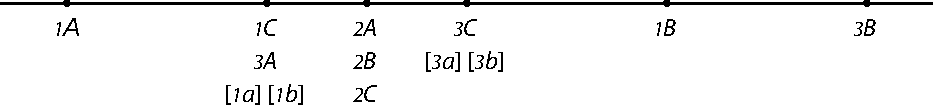
\includegraphics[width=1.0\textwidth]{gesamttex/edit_VIII,3/images/LH_37_05_148-149_d3_149v.pdf}} 
    \vspace{0.2em}
\centerline{\lbrack\textit{Fig.~3}\rbrack}
% \newpage%
  \vspace{1em}
\pstart
\edtext{}{\lemma{\hspace*{1,6mm}\lbrack\textit{Fig.~3}\rbrack}\killnumber\Cfootnote{In Leibnizens Zeichnung fallen die Punkte \textit{{\scriptsize 3}a} und \textit{{\scriptsize 3}b}, entgegen der Definition im Text, mit \textit{{\scriptsize 3}C} zusammen; die Punkte \textit{{\scriptsize 1}a} und \textit{{\scriptsize 1}b} befinden sich in der Umgebung von \textit{{\scriptsize 1}B}. Die Positionen dieser Punkte ändert Hrsg.}}%
%
Si \edlabel{37_05_148-149_6b} $\overset{\displaystyle A, B}{\textup{corporum}}$ in eadem $\overset{\displaystyle ACB}{\textup{recta}}$ uniformiter motorum dentur loca $\overset{\displaystyle {\scriptstyle \textit{2}}A, {\scriptstyle \textit{2}}B}{\textup{praesentia}}$, et 
% =
ante datum tempus $\overset{\displaystyle {\scriptstyle \textit{1}}A, {\scriptstyle \textit{1}}B}{\textup{praeterita}}$; 
\protect\rule[0cm]{0mm}{19pt}invenientur loca eorum post aequale dato tempus $\overset{\displaystyle {\scriptstyle \textit{3}}A, {\scriptstyle \textit{3}}B}{\textup{futura}}$ hoc 
% =
\edtext{modo. Centrum}{\lemma{modo.}\Bfootnote{\textit{(1)}~Cum via c \textit{(2)}~Sumatur a \textit{(3)}~Sumatur \textbar\ in eadem recta \textit{erg.}~\textbar\ punctum quod a centro gravitatis praesenti aeque \textbar\ absit \textit{streicht Hrsg.}~\textbar\ ac centrum gravitatis procedens hinc \textit{(4)}~Centrum~\textit{L}}}
%
\protect\rule[0cm]{0mm}{19pt}eorum gravitatis\protect\index{Sachverzeichnis}{centrum gravitatis} $\overset{\displaystyle {\scriptstyle \textit{3}}C}{\textup{futurum}}$, tantum aberit
% =
a $\overset{\displaystyle {\scriptstyle \textit{2}}C}{\textup{praesente}}$ in contrariam partem in eadem recta, 
\protect\rule[0cm]{0mm}{19pt}quantum $\overset{\displaystyle {\scriptstyle \textit{1}}C}{\textup{praeteritum}}$. Ab hoc 
% =
centro gravitatis\protect\index{Sachverzeichnis}{centrum gravitatis} $\overset{\displaystyle {\scriptstyle \textit{3}}C}{\textup{futuro}}$ hoc modo invento, 
%
\edlabel{37_05_148-149_7a}\edtext{}{% C-Footnote (rechts und links) um B-Footnoten herum
{\xxref{37_05_148-149_7a}{37_05_148-149_7b}}%
\lemma{in partem \lbrack...\rbrack\ sinistri}%
\Cfootnote{Leibniz weicht hier in der Benennung des rechten und linken Körpers sowohl von der Zeichnung als auch von den nachfolgenden Angaben im Text ab.}}% 
\protect\rule[0cm]{0mm}{19pt}\edtext{sumatur in partem dextram distantia corporis}{\lemma{sumatur in partem}\Bfootnote{\textit{(1)}~dextram dis \textit{(2)}~dextram distantia \textit{(a)}~centri \textit{(b)}~corporis~\textit{L}}}
%
dextri a $\overset{\displaystyle \textup{seu}\ {\scriptstyle \textit{3}}A{\scriptstyle \textit{3}}C \sqcap {\scriptstyle \textit{1}}A{\scriptstyle \textit{1}}C}{\textup{centro gravitatis praeterito}}$\protect\index{Sachverzeichnis}{distantia corporis a centrum gravitatis}, et in 
\protect\rule[0cm]{0mm}{19pt}partem sinistram distantia corporis 
% =
$\overset{\displaystyle {\scriptstyle \textit{3}}B{\scriptstyle \textit{3}}C \sqcap {\scriptstyle \textit{1}}B{\scriptstyle \textit{1}}C}{\textup{sinistri ab eodem}}$\protect\index{Sachverzeichnis}{distantia corporis a centrum gravitatis}. Puncta hoc modo inventa erunt loca futura 
\protect\rule[0cm]{0mm}{12pt}quaesita\lbrack,\rbrack\ illud corporis
% =
dextri hoc sinistri.\edlabel{37_05_148-149_7b}
\pend \pstart
\protect\rule[0cm]{0mm}{12pt}In literis ${\scriptstyle \textit{1}}C{\scriptstyle \textit{2}}C \sqcap {\scriptstyle \textit{2}}C{\scriptstyle \textit{3}}C$ et ${\scriptstyle \textit{1}}C{\scriptstyle \textit{3}}C \sqcap {\scriptstyle \textit{1}}C{\scriptstyle \textit{2}}C+{\scriptstyle \textit{2}}C{\scriptstyle \textit{3}}C$.\pend \pstart
% = 
${\scriptstyle \textit{3}}A{\scriptstyle \textit{3}}C \sqcap {\scriptstyle \textit{1}}A{\scriptstyle \textit{1}}C$. ${\scriptstyle \textit{3}}B{\scriptstyle \textit{3}}C \sqcap {\scriptstyle \textit{1}}B{\scriptstyle \textit{1}}C$. \pend \pstart
Haec regula vera est, etiam nullo existente
%
\edlabel{37_05_148-149_8a}\edtext{}{% NEUER ABSATZ UND VARIANTEN – "concursu."
{\xxref{37_05_148-149_8a}{37_05_148-149_8b}}%
\lemma{concursu.}%
\Bfootnote{\textit{(1)}~Ponamus jam exemplum \textit{(2)}~Haec~\textit{L}}}% 
concursu\protect\index{Sachverzeichnis}{concursus}.
\pend \pstart
Haec \edlabel{37_05_148-149_8b} regula intelligi debet de eo casu, quo corpora si concurrunt
% =
perfecte dura aut Elastica\protect\index{Sachverzeichnis}{corpus perfecte durum aut elasticum} sunt. Sed si non
%
\edtext{sint, tunc}{\lemma{sint,}\Bfootnote{\textit{(1)}~ita cu \textit{(2)}~tunc~\textit{L}}}
%
\protect\rule[0cm]{0mm}{16pt}${\scriptstyle \textit{3}}A{\scriptstyle \textit{3}}C \sqcap \displaystyle\frac{m}{n}{\scriptstyle \textit{1}}A{\scriptstyle \textit{1}}C$
% =
et
${\scriptstyle \textit{3}}B{\scriptstyle \textit{3}}C \sqcap \displaystyle\frac{m}{n}{\scriptstyle \textit{1}}B{\scriptstyle \textit{1}}C$, exprimetque $\displaystyle\frac{m}{n}$ rationem, qua minor est vis resilitionis\protect\index{Sachverzeichnis}{vis resilitionis} a natura
% =
\protect\rule[0cm]{0mm}{10pt}materiae, quam posita
%
\edtext{perfecta duritie}{\lemma{perfecta}\Bfootnote{\textit{(1)}~soliditate esse deberet \textit{(2)}~duritie~\textit{L}}} aut restitutione\protect\index{Sachverzeichnis}{durities vel restitutio perfecta} esse
%
\edtext{deberet. Porro}{\lemma{deberet.}\Bfootnote{\textit{(1)}~Applicemus regulam nostram uni casui. \textit{(2)}~Porro~\textit{L}}}
%
facile demonstratur regula 
% =
nostra, quia eadem est via navis\protect\index{Sachverzeichnis}{navis} et centri gravitatis\protect\index{Sachverzeichnis}{via centri gravitatis}, in navi\protect\index{Sachverzeichnis}{navis} feruntur corpora celeritate \textit{{\scriptsize 1}A{\scriptsize 1}C}\lbrack,\rbrack\ % =
\textit{{\scriptsize 1}B{\scriptsize 1}C}, et posita perfecta duritie vel restitutione\protect\index{Sachverzeichnis}{durities vel restitutio perfecta}, eadem celeritate 
%
\edtext{redeuntur, portantur}{\lemma{redeuntur,}\Bfootnote{\textit{(1)}~adde \textit{(2)}~portantur~\textit{L}}}
%
autem
% =
et cum navi\protect\index{Sachverzeichnis}{navis}, intelligentur ergo transferri ex $\overset{\displaystyle {\scriptstyle \textit{2}}A}{\underset{\displaystyle {\scriptstyle \textit{2}}C}{{\scriptstyle \textit{2}}B}}$
%
\edtext{in \textit{{\scriptsize 3}C}}{\lemma{in}\Bfootnote{\textit{(1)}~$\protect\overset{\displaystyle {\scriptstyle \textit{3}}A}{{\scriptstyle \textit{3}}B}$ \textit{(2)}~\textit{{\scriptsize 3}C}~\textit{L}}} cum navi\protect\index{Sachverzeichnis}{navis}, et praeterea \edtext{pecul\lbrack i\rbrack ari}{\lemma{}\Bfootnote{peculari \textit{L ändert Hrsg.}}} motu\protect\index{Sachverzeichnis}{motus peculiaris} 
% =
aut 
\protect\rule[0cm]{0mm}{10pt}progredi aut regredi intelligentur. Sed quia hoc  
%
\edtext{modo pro}{\lemma{modo}\Bfootnote{\textit{(1)}~ut \textit{(2)}~pro~\textit{L}}}
%
punctis sumuntur corpora, ideo et
% =
ponendo \textit{{\scriptsize 2}C} differre a \textit{{\scriptsize 2}A} et a \textit{{\scriptsize 2}B} eaque differre inter se,  
%
\edtext{tunc regula}{\lemma{tunc}\Bfootnote{\textit{(1)}~sumemus \textit{(2)}~regula~\textit{L}}}
%
haec erit: in partes oppositas a
% =
\edtext{\textit{{\scriptsize 3}C}, sumatur \textit{{\scriptsize 2}A{\scriptsize 3}a}}{\lemma{\textit{{\scriptsize 3}C}, sumatur}\Bfootnote{\textit{(1)}~\textit{{\scriptsize 2}A{\scriptsize 3}A} \textit{(2)}~\textit{{\scriptsize 2}A{\scriptsize 3}a}~\textit{L}}}, item ${\scriptstyle \textit{2}}B{\scriptstyle \textit{3}}b\, \sqcap\, {\scriptstyle \textit{2}}C{\scriptstyle \textit{1}}C$ 
%
\edtext{et a sinistro}{\lemma{et a}\Bfootnote{\textit{(1)}~dextro ip \textit{(2)}~sinistro~\textit{L}}}
%
ipsius \edtext{\textit{{\scriptsize 3}b} sumatur}{\lemma{}\Bfootnote{\textit{{\scriptsize 3}b} \textbar\ sumatur \textit{streicht Hrsg.}~\textbar\ sumatur~\textit{L}}} 
%
${\scriptstyle \textit{3}}b{\scriptstyle \textit{3}}B \sqcap {\scriptstyle \textit{1}}B{\scriptstyle \textit{1}}b$ (posito \textit{{\scriptsize 1}b} locum in quo esset \textit{B}, si corpora celeritatibus reciprocis\protect\index{Sachverzeichnis}{celeritas reciproca} concurrerent) 
% =
et in dextrum
%
${\scriptstyle \textit{3}}a{\scriptstyle \textit{3}}A \sqcap {\scriptstyle \textit{1}}A{\scriptstyle \textit{1}}a$ (posito eodem de \textit{{\scriptsize 1}a}) et habebuntur \textit{{\scriptsize 3}B}, \textit{{\scriptsize 3}A}, sed nota videntur
% =
destrui illa exigua \textit{{\scriptsize 1}C{\scriptsize 1}a}, \textit{{\scriptsize 1}C{\scriptsize 1}b}, \textit{{\scriptsize 3}a{\scriptsize 3}C}, \textit{{\scriptsize 3}b{\scriptsize 3}C}, ideo regula initio assignata subsistet.
\pend \pstart
\lbrack148~r\textsuperscript{o}\rbrack\
\edlabel{37_05_148-149_11a}Applicemus exemplo. Sit corpus \textit{A} triplum ipsius \textit{B}, celeritates vero sint aequales.\pend \pstart
% =
${\scriptstyle \textit{1}}A{\scriptstyle \textit{1}}C \sqcap 1$, ${\scriptstyle \textit{1}}C{\scriptstyle \textit{1}}B \sqcap 3$, ${\scriptstyle \textit{1}}C{\scriptstyle \textit{2}}C \sqcap 1 \sqcap {\scriptstyle \textit{2}}C{\scriptstyle \textit{3}}C$. ${\scriptstyle \textit{3}}C{\scriptstyle \textit{3}}A \sqcap {\scriptstyle \textit{1}}C{\scriptstyle \textit{1}}A$, ${\scriptstyle \textit{3}}C{\scriptstyle \textit{3}}B \sqcap {\scriptstyle \textit{1}}C{\scriptstyle \textit{1}}B$.
% =
\pend
%%%%%%%%%%%%%%%%%%%%%%%%%%%%%%% FIG. 5 %%%%%%%%%%%%%%%%%%%%%%%%%%%%
\vspace{1.5em}
  \centerline{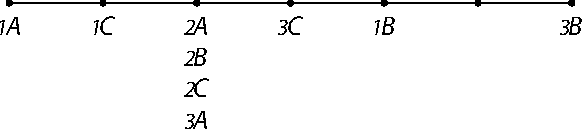
\includegraphics[width=0.66\textwidth]{gesamttex/edit_VIII,3/images/LH_37_05_148-149_d4_148r.pdf}} 
    \vspace{0.5em}
\centerline{\lbrack\textit{Fig.~4}\rbrack}
% \newpage%
  \vspace{1.0em}
\pstart
Sed ita perditur potentia\protect\index{Sachverzeichnis}{potentia}:\pend \pstart
% =
\edtext{Nam corpus}{\lemma{Nam}\Bfootnote{\textit{(1)}~fiet \textit{(2)}~corpus~\textit{L}}}
%
$A \sqcap 3$, corpus 
%
\edtext{$B \sqcap 1$. Celeritas}{\lemma{$B \sqcap 1$.}\Bfootnote{\textit{(1)}~Potentia \textit{(2)}~Celeritas~\textit{L}}}
%
eorum aequalis sit 2. Erit corporis \textit{A} potentia\protect\index{Sachverzeichnis}{potentia} 6,
% =
corporis \textit{B} potentia\protect\index{Sachverzeichnis}{potentia} 2, ante concursum\protect\index{Sachverzeichnis}{concursus} summa 8.
% =
Post concursum\protect\index{Sachverzeichnis}{concursus} corporis \textit{A} potentia\protect\index{Sachverzeichnis}{potentia} erit 0, quia non 
% =
movetur, corporis \textit{B} celeritas est dupla prioris nempe
% =
4, ergo potentia\protect\index{Sachverzeichnis}{potentia} ejus erit 4. Ergo in summa potentia\protect\index{Sachverzeichnis}{potentia} 
% =
erit 4, cum debeat  
%
\edtext{esse 8. Ergo}{\lemma{esse 8.}\Bfootnote{\textit{(1)}~Vidi \textit{(2)}~Videtur \textit{(3)}~Ergo~\textit{L}}}
%
\edlabel{37_05_148-149_10a}regula
% =
\edtext{nostra per}{\lemma{nostra}\Bfootnote{\textit{(1)}~quae \textit{(2)}~per~\textit{L}}}
%
compositiones\lbrack,\rbrack\protect\index{Sachverzeichnis}{regula per compositiones}\edlabel{37_05_148-149_10b}
%
\edtext{quae Hugenianae\protect\index{Sachverzeichnis}{regula Hugeniana}\protect\index{Namensregister}{\textso{Huygens} (Hugenius, Ugenius, Hugens, Huguens), Christiaan 1629\textendash1695} coincideret,}{\lemma{quae Hugenianae coincideret}%
\Cfootnote{
\protect\index{Namensregister}{\textso{Huygens} (Hugenius, Ugenius, Hugens, Huguens), Christiaan 1629\textendash1695}\textsc{C.~Huygens}, \cite{00529}\glqq Regles du mouvement dans la rencontre des corps\grqq, \cite{00157}\textit{JS} (Pariser Ausgabe), 18.~März 1669, S.~22\textendash24 (\cite{00113}\textit{HO} XVI, S.~179\textendash181), bes.~§4. Vgl.\ auch Leibnizens kommentierte Auszüge von März\textendash Mai 1677 (N.~\ref{RK57267-2}).}}
%
 utique mutanda est
% =
et per compositiones quidem indaganda 
%
est directio\protect\index{Sachverzeichnis}{directio celeritatis}
%
et proportio celeritatum\protect\index{Sachverzeichnis}{proportio celeritatum}, sed
% =
quantitas absoluta\protect\index{Sachverzeichnis}{quantitas absoluta celeritatis} sumenda est talis ut sit eadem quae ante potentia\protect\index{Sachverzeichnis}{potentia}. Itaque movebitur
% =
\textit{B}, hoc casu celeritate 
%
\edtext{ut 8. Si}{\lemma{ut 8.}\Bfootnote{\textit{(1)}~Hinc via videtur excogitari posse, \textit{(2)}~Si~\textit{L}}}
%
secus, tunc videtur
% =
via excogitari posse ope ejusmodi compositionum efficiendi perennem motum\protect\index{Sachverzeichnis}{motus perennis}. Verum
% =
tunc non id obtinemus, ut eadem via incedat centrum gravitatis\protect\index{Sachverzeichnis}{via centri gravitatis}, neque etiam ut eadem semper
% =
sit corporum distantia\protect\index{Sachverzeichnis}{distantia corporum}. Ergo rursus in difficultates revoluti sumus. Nimirum si ponamus
% =
corpus aliquod ferri in navi\protect\index{Sachverzeichnis}{navis} celeritate aliqua, et navim\protect\index{Sachverzeichnis}{navis} ferri aequali contraria\protect\index{Sachverzeichnis}{celeritas aequalis contraria}, perinde est ac
% =
si corpus istud nullam haberet potentiam\protect\index{Sachverzeichnis}{potentia}.\edlabel{37_05_148-149_11b}
\pend
\pstart
\lbrack148~v\textsuperscript{o}\rbrack\
Ex his duobus quod centrum gravitatis\protect\index{Sachverzeichnis}{centrum gravitatis} in eadem procedit recta
% =
et quod eadem manet semper
% =
distantia\protect\index{Sachverzeichnis}{distantia} determinantur omnia.
\pend
%%%%%%%%%%%%%%%%%%%%%%%%%%%%%%% FIG. 6 %%%%%%%%%%%%%%%%%%%%%%%%%%%%
\vspace{2.0em}
  \centerline{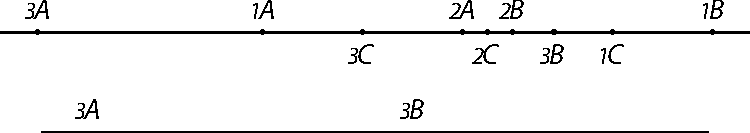
\includegraphics[width=0.75\textwidth]{gesamttex/edit_VIII,3/images/LH_37_05_148-149_d5_148v.pdf}} 
    \vspace{0.5em}
\centerline{\lbrack\textit{Fig.~5}\rbrack}
% \newpage%
  \vspace{1.5em}
 \pstart
Datur punctum \textit{{\scriptsize 3}C}, datur et
%
$\displaystyle\frac{{\scriptstyle \textit{3}}B{\scriptstyle \textit{3}}C}{{\scriptstyle \textit{3}}A{\scriptstyle \textit{3}}C}\, \sqcap\, \displaystyle\frac{y}{x}$ \edtext{$\sqcap\, \displaystyle\frac{a}{b}$}{\lemma{}\Bfootnote{$\sqcap\ \displaystyle\frac{a}{b}$ \textit{erg.}~\textit{L}}}, 
%
datur et
% =
$y+x\, \sqcap\, e+f$.
%
Ergo $y\, \sqcap\, e+f-x\, \sqcap\, \displaystyle\frac{a}{b}x$.
%
\protect\rule[0cm]{0mm}{18pt}\edtext{$e+f \sqcap d$, $a+b \sqcap s$.}{\lemma{}\Bfootnote{$e+f \sqcap d$, $a+b \sqcap s$. \textit{erg.}~\textit{L}}} 
%
Ergo $\displaystyle\frac{be+bf}{a+b} \sqcap x$.
%
Et $\displaystyle\frac{ae+af}{a+b}x\edtext{\sqcap y$. Seu}{\lemma{$\sqcap\ y$.}\Bfootnote{\textit{(1)}~Ergo ambo reperent \textit{(2)}~\textbar\ Si \textit{streicht Hrsg.}~\textbar\ \textit{(3)}~Seu~\textit{L}}}
%
$x \sqcap \displaystyle\frac{bd}{s}$, $y \sqcap \displaystyle\frac{ad}{s}$.
$a+b \sqcap s$. $y+x \sqcap d$. $\displaystyle\frac{y}{x} \sqcap \displaystyle\frac{s-b}{b} \sqcap \displaystyle\frac{a}{s-a}$.
Ergo
$\displaystyle\frac{y+x \sqcap d}{x} \sqcap \displaystyle\frac{s - b + b}{b}$. Ergo $\displaystyle\frac{x}{d} \sqcap \displaystyle\frac{b}{s}$.
\protect\rule[0cm]{0mm}{18pt}Ita res demonstratur
\protect\rule[0cm]{0mm}{10pt}lineariter.
\pend
\count\Afootins=1200%
\count\Bfootins=1200%
\count\Cfootins=1200